\documentclass{article}
\usepackage{graphicx}
\usepackage{hyperref}

\usepackage{tikz}
\usepackage[default]{lato}
\usepackage[T1]{fontenc}
\usepackage{titlesec}
\usepackage{titling}
\usepackage[hmargin=0.5in,bmargin=1in,tmargin=1in,centering]{geometry}
\usetikzlibrary{shadows.blur}
\usetikzlibrary{shapes.symbols}
\usetikzlibrary{positioning,fit,hobby}

% The red used throughout the document
\definecolor{red}{HTML}{D32D2D}
\pagenumbering{gobble}  

% Defines the red lines at the top and bottom of each page
\newcommand\AddLines{%
\begin{tikzpicture}[remember picture,overlay]
    \fill[red] (current page.north west) rectangle ([yshift=-2mm]current page.north east);
    \fill[red] (current page.south west) rectangle ([yshift=2mm]current page.south east);
    \end{tikzpicture}%
}

% Adds the red lines to each page
\AtBeginShipout{\AddLines}
\AtBeginShipoutFirst{\AddLines}

% Defines the red block for section titles
\newcommand\SecTitle[1]{%
\begin{tikzpicture}
  \node[inner ysep=1cm,text width=\paperwidth,fill=red,text=white,font=\Huge]  at (0,0) 
 {\parbox{0.4in}{\mbox{}}\parbox{\dimexpr\textwidth-0.4in\relax}{\raggedright\strut#1\strut}\parbox{0pt}{\mbox{}}};
\end{tikzpicture}%
}

% Adds the red block to section titles
\titleformat{\section}{\normalfont}{}{-0.5in}{\SecTitle}

% NO MORE INDENTS
\setlength\parindent{0pt}
\title{Computational Graphing}

\begin{document}
    \newcommand{\titleimage}{compiax.png}
    \tikzstyle{title}=[font=\fontsize{32}{144}\selectfont]
\tikzstyle{date}=[font=\fontsize{30}{144}\selectfont]
\tikzstyle{subtitle}=[font=\fontsize{20}{144}\selectfont, white]
\begin{titlepage}        
        \begin{tikzpicture}[remember picture,overlay, anchor = west]
            % Graphic
            \node at (-1.5,-16) {\includegraphics[width=\paperwidth]{\titleimage}};
            
            % Header
            \fill[red] (current page.north west) rectangle ([yshift=-8cm]current page.north east);
            \node[title] (title) at (-0.5,0) {\thetitle};
            \draw[line width=0.75mm, white] ([yshift=-1cm]title.west) -- ([yshift=-1cm]title.east);
            \node[subtitle] at ([yshift=-1.6cm, xshift=-2.4cm]title.east) {Tender};
            
            % Logos
            \node at (-0.8,-22.5)
            {
\includegraphics[width=4cm]{../Common/UniversityOfPretoriaLogo.png}};
            \node at (15,-23.3) {
\includegraphics[width=5cm]{../Common/AlbertPrimeLogo.png}};  
            
            % Hexagon
            \draw[line width=1mm, white] (14.4,-5.1) -- (14.4,-4) -- (16.4,-2.75) -- (18.4,-4) -- (18.4,-5.1);
            \node[date, white] at (15.05,-4.5) {May};
            \draw[line width=1mm, red] (14.4,-5.1) -- (14.4,-6.35) -- (16.4,-7.6) -- (18.4,-6.35) -- (18.4,-5.1);
            \node[date, red] at (15.1,-6) {2017};
            
        \end{tikzpicture}        
    \end{titlepage}

    
    % Styles
\tikzstyle{table_number}=[white,font=\fontsize{80}{144}\selectfont]
\tikzstyle{table_heading}=[font=\fontsize{35}{144}\selectfont,text width = 14cm]

\begin{tikzpicture}[remember picture,overlay, anchor = north]
    % Clear footer and header
    \fill[white] ([xshift=5.8cm]current page.north west) rectangle ([yshift=-3mm]current page.north east);
    \fill[white] ([xshift=5.8cm]current page.south west) rectangle ([yshift=3mm]current page.south east);   
    % Sidebar and Title
    \fill[red] (current page.north west) rectangle ([xshift=5.8cm]current page.south west);
    \node[title] at (7,0) {Table of Contents};         
\end{tikzpicture}
    % Entries in the contents page
    \begin{tikzpicture}[remember picture,overlay,anchor = north]
        % Project Overview
        \node[table_number] at (2.5,-3) {2};
        \node[table_heading] at (10.5,-3.5) {Project Overview};
        % Methodologies
        \node[table_number] at (2.5,-6) {3};
        \node[table_heading] at (10.5,-6.5) {Methodologies};
        % The Team
        \node[table_number] at (2.5,-9) {4};
        \node[table_heading] at (10.5,-9.5) {The Team}; 
    \end{tikzpicture}
	
	\pagenumbering{arabic}

	\newpage

	\section{Project Overview}

	Our vision of this project is a very easy to use, web based, interpreted programming language. We see this tool as a way for people, 
    who may not be able to code, to write there own, short mathematical programs. It is important that this part of the tool be treated as
    any interpreter program would. Implementing typical interpreter components, such and lexical analysis and syntax analysis, is important
    to ensure that the libraries and packages, written by the user, preform in a reliable and consistant manner, such that the user can 
    trust whatever output their functions return. Our plan is try and write the interpreter in such a way that it can be run in either python
    or javascript on the client's side, to ensure that output is produced and displayed as fast as possible, as well as remove pressure 
    from the server. However, we do see this interpreter possibly getting to larger to pass through to the client, depending on what 
    funcationality is already implemented for the user (mathimatical operations, control structures, etc.), so running the interpreter on the
    server side may be the best option inorder to keep the web tool light weight. \par

    It is also extremely important that the web tool is easy to learn and use, as it will be used primarily by people who do not necessarily
    understand computer programming. We do not want to over whelm new users with too many options that they may not understand, but at the 
    same time we do want to provide them with all the tools that they could possibly need to create any function, as well as provide them 
    with any all the information, about their libraries, that they could need. This is where we see UI design being important. We will need 
    to create the website in such as way that users will be able to find whatever they may want easily and without getting confused and 
    frustated. Our team fully believes in good, intuitive GUI design that will make the users feeling comfortable when using our software.
    We would like to make use of a popular html/css framework, such as materialize css, to give the final product a very clean and modern look,
    well also speeding up our production time. We would also plan to do multiple usability tests towards the end of our development, to ensure
    that potential users will feel comfortable, and that we have succeeded in making the application intuitive for the users. \par

    It is important that all user information be stored in a safe an effient manner on the back-end, and that information retrieval be fast. 
    That is why we propose making use of the MEAN stack when creating the server and database. The MEAN stack will allow us to create a fast, 
    custom, webserver to handle and request that the user may have. Such requests would include, logging into the users account, fetching 
    libraries that the user may currently be working on, exploring other users libraries and profiles, etc. A mongo database will allow for 
    extremely fast data retrieval allowing the server to respond to more requests in a shorter time than a LAMP stack implementation. A MEAN 
    stack implemenation will allow us create a seperate gateway for exnternal components to access the libraries created by uses, as mentioned
    in the orignal brief.\par

    A possible potential feature that we would like to add to this tool, is the ability to download libraries and packages as a java/c++/python 
    class. The user would simply create and test the library on the web application and then select an option to download it as a prograaming
    language class. The library would then be sent to the node.js server, which would translate the graph into a class, and return the file to 
    the user. Users could also download any public libraries that someone else has implemented, to use in their own programs. The would not be 
    such a tough feature to implement if we treat this application as an interpreter, as we will just be translating code. This feature will 
    allow programmers the ability to quickly write and test mathematical functions which they can the use in their programs. This could help 
    attract more users which a different skill set to the site. \\
    \\
    \noindent\textbf{The following is our proposed deployment of the system} \\
    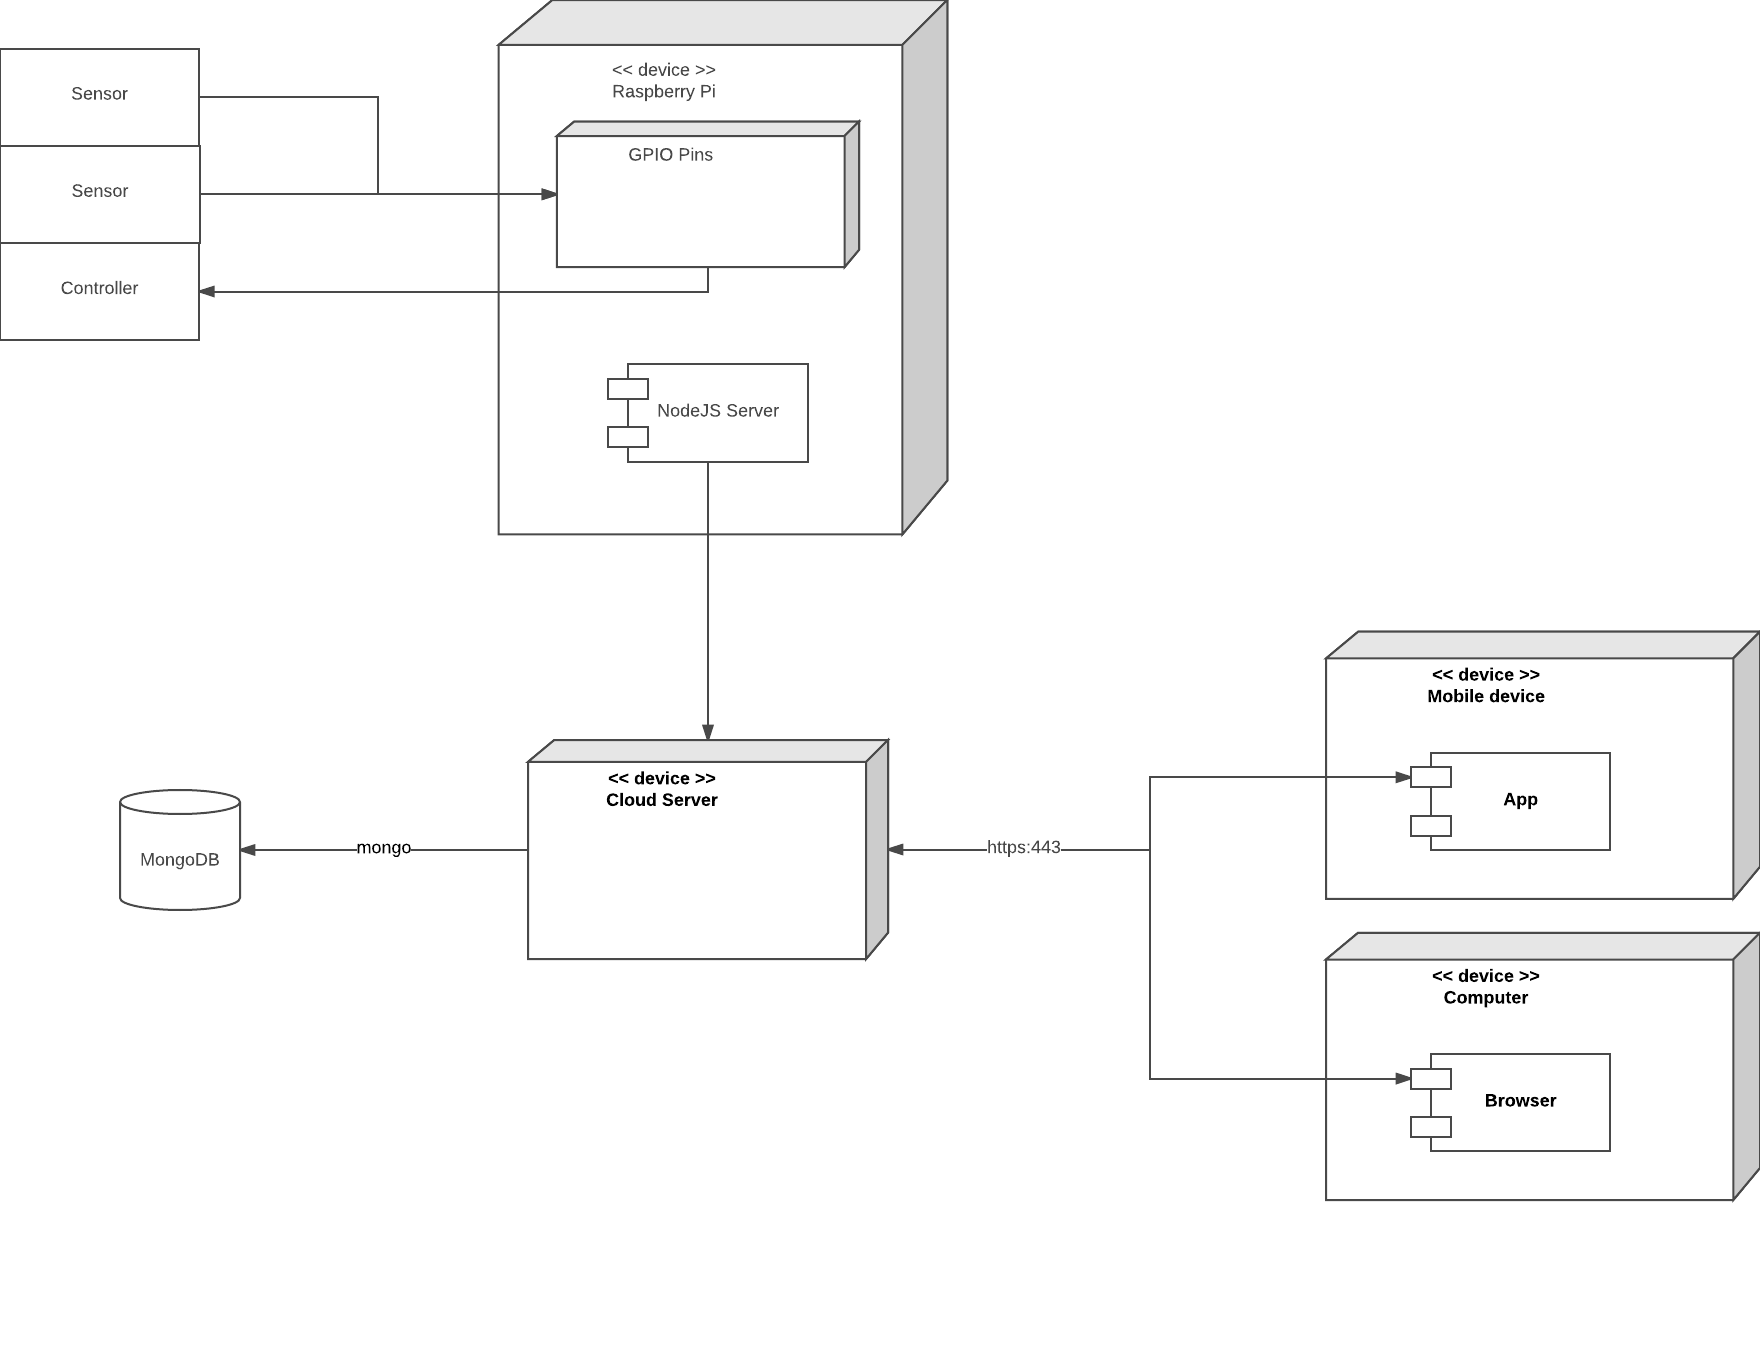
\includegraphics[width=\textwidth]{deployment}

	\newpage
	\section{Proposed Methodology}
	 Praesent vel eros et metus imperdiet elementum eget gravida urna. Duis turpis diam, tempor vitae enim vitae, fermentum congue elit. Duis vitae scelerisque metus, et laoreet turpis. Nulla malesuada ligula ut suscipit vestibulum. In at iaculis urna. Mauris et dapibus nulla, ut auctor arcu. In consequat mollis sem sit amet viverra. Duis ante nulla, rutrum et mollis sed, condimentum at neque. Donec in leo eget massa gravida vestibulum. Praesent consequat turpis et tellus porta placerat. Ut mattis tempus tempor. Nullam vel elit vel nibh convallis consequat. Mauris consequat eros elit, ut maximus odio feugiat et. Praesent sed consectetur arcu.

In hac habitasse platea dictumst. Sed dictum vulputate molestie. Fusce placerat justo sed sem ullamcorper, a dictum ante mollis. Ut nisi augue, rutrum sit amet odio eget, ultricies maximus ex. Fusce finibus et metus sed elementum. Aenean at lacus nec nunc dignissim fringilla. Pellentesque placerat interdum iaculis. Curabitur finibus elit ac tincidunt aliquam. 
	\newpage
	\section{The Team}
	\textbf{Dimpho Mahoko} \\
	I am an aspiring software developer looking to gain new skills and develop those I already have. Notable skills include web development, Java, C++, JavaScript, PHP, HTML  \\ \\ %Should I list ALLLLLLLLLL My Skils????? I mean like ALLLLLLLLLL of them?????? Because I don't think we have enough time. Jokes. Seriously though. ALL the languages seems a bit tedious and also saying javascript does'nt imply node, angular and so on so should I add those too.  \\
	 Below are my accomplishments worth mentioning in no particular order.
	\begin{itemize}
		\item Second place in the Standard Bank IT challenge finals in 2016.\\
	
		\item Webmaster at Tuks FM from September 2016 till present. \\ 
			Responsibilities include maintaining the website and keeping it up to date. \\
			
		\item Mentor at The University of Pretoria EBIT Week for EBIT Marketing \\
			Responsibilities include database administration, website maintenance and all other admin related responsibilities like communication with parents whose children wish to attend EBIT Week. \\
			
		\item 2016 Retro Rabbit Rabbiteer program attendee \\
			The program was focused mainly on giving programming students an idea of how work in the industry is actually done. Notable technologies learnt include GitHub integration with team work and cloud computing and hosting. \\%I'll elaborate further
	\end{itemize}
	

\textbf{Jason van Hattum}\\ 
    I am a motivated developer with a passion for application and web-app development. Technologies that I am fluent in include full-stack MEAN and LAMP development, Java, C++, Android, Python and Django. I have experience in project management, web-app development and Android application development. \\
    
    I enjoy experimenting in my free time, especially working on side projects on my Raspberry Pi and building Android applications. I also enjoy making graphical programs in WebGL. My hobbies also include reading, playing games, and fishing. \\
    
    \noindent
    Projects that I have worked on include:
    \begin{itemize}
        \item A web application for the University of Pretoria used for peer-review and team evaluation within major projects (Can be found \href{https://github.com/teampinocchio/pinocchio/wiki}{\underline{here}}.). Skills that I developed here include front-end languages such as HTML, CSS, and Javascript; Python and Django.
    
        \item A variety of Android applications as a freelancing developer, both front-end and back-end. Skills developed here include Android development, Google Firebase, interface design and NodeJS.
    \end{itemize}
    
    \noindent
	Accomplishments and work experience:
    \begin{itemize}
        \item A member of the Golden Key International Honors Society.
        \item A teaching assistant and tutor for multiple subjects since January 2016.
        \item Participated in the Standard Bank IT Challenge in 2016 and 2017; and ACM in 2016.
        % \item Passed AI
        % \item Got destroyed in the Digital Gaming League, Dota division.
    \end{itemize}

\textbf{Kyle Erwin}\\
	Currently studying a BSc Computer science. I'm a well rounded programmer with many skills in many languages. My passion lies in artificial intelligence and creating applications with an intuitive design. I'm a harder worker that is known to be ``on top of things`` by my peers. \\ 

	I've worked in many leader positions and understand the importance of synergy in a team. Most noteworthy, I was apart of the TukVillage residence committee and the graphic desiner for all of the events (2015 - 2016). I launched a web development company, \href{www.unhinged.co.za}{\underline{unhinged.co.za}}, with team member Keagan Ferrett. My work has also extended to app development and partnerships with small startup companies.\\

	In my free time I often find myself programming on personal projects, coming up with new concepts and focusing my time on perfection my artificial intelligence skills. 

	\noindent
	More about me and my skills:
    \begin{itemize}
        \item Up-to-date with all the latest design trends.
        \item Used applications such as google analytics, webmaster and google trends. 
        \item Written many C++ tutorials for beginner programmers
        \item Business skills and working with clients. 
        \item An understanding of scala, a programming language great for AI. 
    \end{itemize}

    \end{itemize}
\textbf{Joshua Cilliers}\\
Lorem ipsum dolor sit amet, consectetur adipiscing elit. Curabitur aliquam augue a odio cursus bibendum. Suspendisse felis diam, varius eu molestie quis, condimentum eget libero. Fusce egestas ligula sit amet metus vehicula ornare. Integer et magna sapien. Pellentesque nec metus in sapien congue gravida eu quis dolor. Maecenas consequat nunc a enim ullamcorper venenatis. Suspendisse at faucibus dolor, imperdiet rhoncus ante. \\ \\
\textbf{Keegan Ferrett}\\
Lorem ipsum dolor sit amet, consectetur adipiscing elit. Curabitur aliquam augue a odio cursus bibendum. Suspendisse felis diam, varius eu molestie quis, condimentum eget libero. Fusce egestas ligula sit amet metus vehicula ornare. Integer et magna sapien. Pellentesque nec metus in sapien congue gravida eu quis dolor. Maecenas consequat nunc a enim ullamcorper venenatis. Suspendisse at faucibus dolor, imperdiet rhoncus ante.

\end{document}


	\section{Why Albert Prime?}

    Two of our memembers have both completed the compiler construction course at the University of Pretoria, and will be able to apply 
    the knowledge gained from building a compiler into building the necessary components needed for the interpreter component of this project. 
    It is important that this is done correctly to ensure that no unexpected errors or crashes occur when a user is testing their 
    created library. Although this may be seen as a very basic interpreter, it will still be important to implement all the necessary 
    components of an interpreter/compiler to ensure that, even as functions and projects get larger, the user can still be sure that they are
    getting reliable and consistant results, without running the risk of potentially crashing the node.js server. It will also give us the 
    ability of being able to add more basic, such as if statements and loops, with little effort.\par

    Every member of our team has experience with working on front-end and back-end web development. This is necessary for this project 
    as our vision for the final product would involve much of what the user is seeing, being done on the client's side, as well as having
    admistrative tasks, being worked on on the back-end. The front-end needs aesthetically pleasing as well as being easy to use and intuitive,
    well the back-end needs to be secure, safe, and reliable to ensure that no personal data is lost and that the web server stays up 
    and running at all times. Each member has experience working with the MEAN stack giving us the advantage of not needing to relearn the
    the thechnologies used in a MEAN stack implementation.\par

    Finally, each member of our team is a skilled mathematician, having completed calculus, linear algebra, and discrete mathematics courses.
    This means we will not have any trouble implementing and testing the mathematical logic. We will be able to account of any possible need
    that a user may have, such as binary mathematics, discrete mathematics, or linear algebra operations.


\end{document}